\section{Durchführung}
\label{sec:Durchführung}

\subsection{Messung bis 1 bar}
Der in \autoref{fig:aufbau1} abgebildete Aufbau wird aufgebaut. Bevor gemessen werden kann muss zuerst mithilfe des Manometers
der Luftdruck und die Temperatur in der entlüftete Apparatur gemessen werden. Zunächst wird die Apparatur mithilfe der 
Wasserstrahlpumpe auf den am niedrigsten zu erreichenden Druck evakuiert. Es werden der Absperrhahn und das Drosselventil geschlossen
und der Merhrhalskolben mit der zu untersuchenden Substanz mithilfe der Heizhaube langsam erhitzt.
Zeitgleich wird das Kühlwasser eingeschaltet, sodass die Einzelteile nicht überhitzen. Bei kontrollierter Erhitzung werden paarweise
Temperatur und Druck gemessen, bis der Druck 1 bar erreicht hat.

\begin{figure}[H]
    \centering
    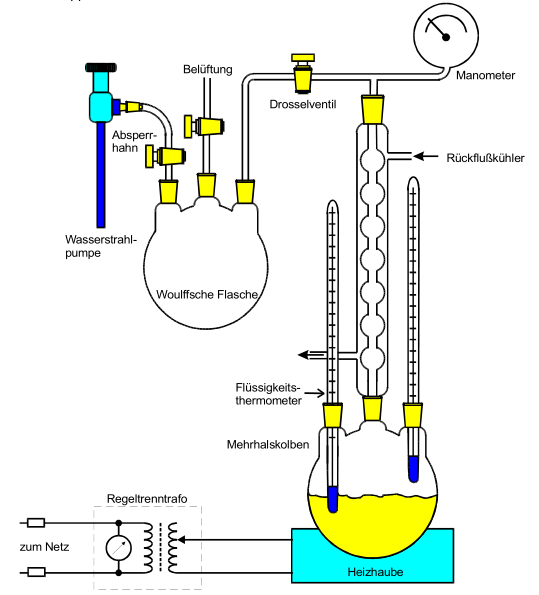
\includegraphics[width=0.75\textwidth]{daten/aufbau1.png}
    \caption{Erster Aufbau \cite{anleitung}.}
    \label{fig:aufbau1}
\end{figure}

\subsection{Messung von 1 bis 15 bar}
Die Verschraubung am Stahlrohr wird geöffnet und der Hohlraum mit der zu untersuchenden Substanz vollständig gefüllt.
Hier ist die zu untersuchende Substanz entgastes und destilliertes Wasser. Die Verschraubung wird nun geschlossen.
Die Apparatur wird nun nach \autoref{fig:aufbau2} vollständig aufgebaut und eingeschaltet. Es wird gewartet bis die Temperatur der zu 
untersuchenden Substanz ungefähr bei $\SI{110}{\celsius}$ aufgeheitzt wurde, da ab jetzt das Druckmessgerät anfangen wird auszuschlagen. 
Es wird der Sättigungsdampfdruck und die dazugehörige Siedetemperatur des Wassers paarweise gemessen.
Die Werte werden jeweils bei einer Erhöhung um 1 bar aufgetragen bis 15 bar erreicht sind.


\begin{figure}[H]
    \centering
    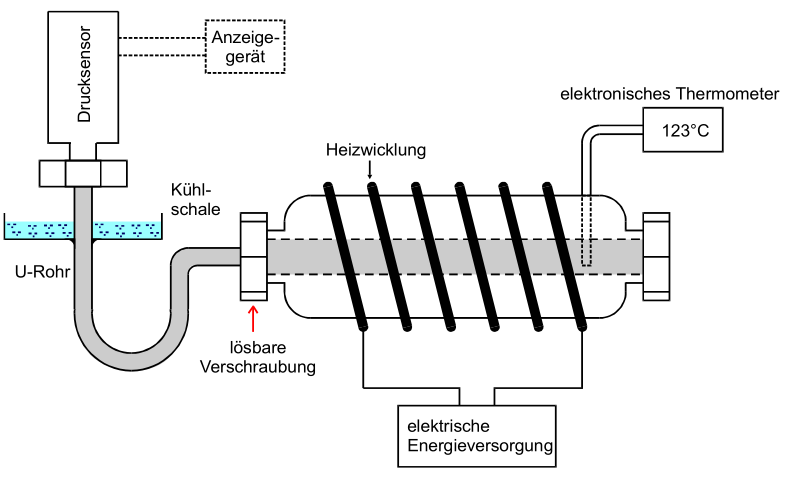
\includegraphics[width=0.75\textwidth]{daten/aufbau2.png}
    \caption{Zweiter Aufbau \cite{anleitung}.}
    \label{fig:aufbau2}
\end{figure}